\documentclass[10pt]{report}


\usepackage[french]{babel}
\selectlanguage{french}
\usepackage[T1]{fontenc}
\usepackage[utf8]{inputenc}
\usepackage{graphicx}
\usepackage[top=2.6cm, bottom=2.6cm, left=2.6cm, right=2.6cm]{geometry}
\usepackage{amsmath}

%\usepackage{siunitx} %Permet d'aligner les nombres sur la virgule, avec le spécificateur de colonne S

\begin{document}
	\large		%Police de taille large
	\sffamily	%Police sans empattement
	%\maketitle
	
	%Page de garde
	\begin{titlepage}
		\begin{sffamily}
			\begin{center}
				
				
\includegraphics[scale=0.25]{insa_cvl_grand_logo.jpg}~	
\includegraphics[scale=0.86]{Logo_ISIR.png}~	
\includegraphics[scale=0.12]{Logo_officiel_de_Sorbonne_Universite.png}~\\[3cm]
				
				\textsc{\huge \textbf{Stage de 4ème année}}\\[1cm]
				\textsc{\LARGE \textbf{Sensor Fusion of IMU and 3d Positioning data for Virtual/Augmented/Mixed Reality
			}}\\[2cm]
				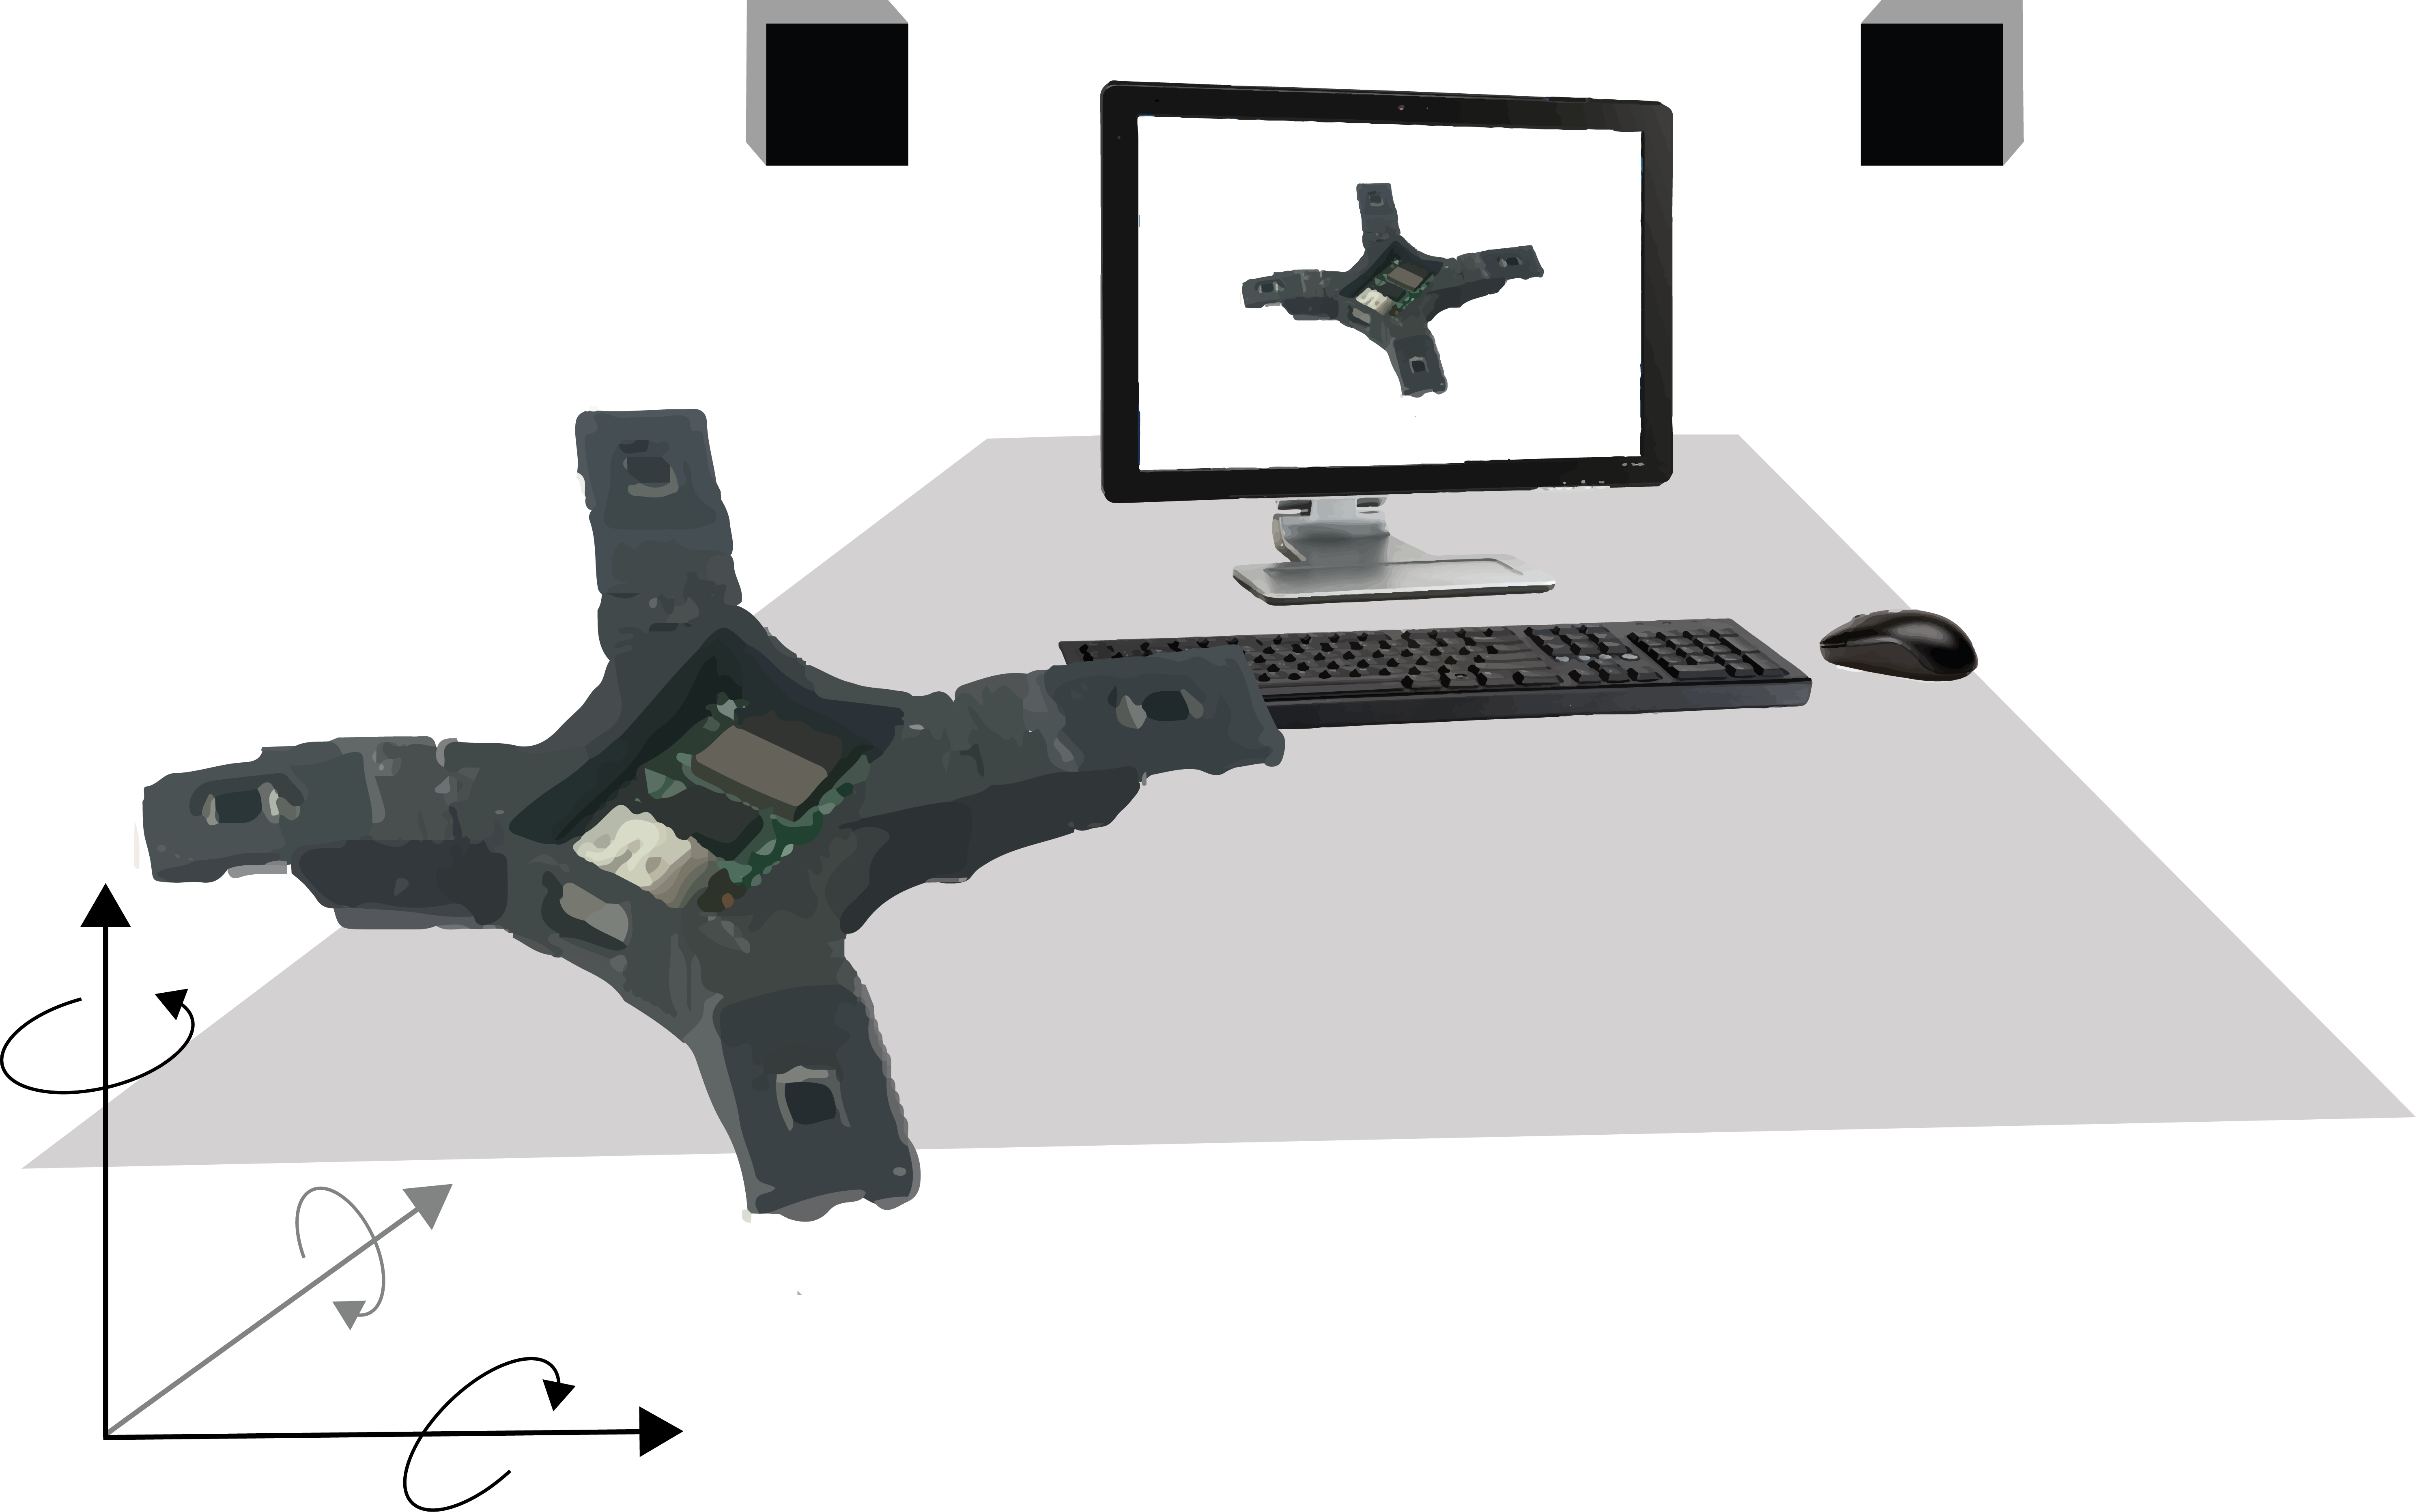
\includegraphics[scale=0.2]{tracker.png}~\\[1cm]
				\Large Par \textbf{Julien \bsc{Mellet}}\\[1cm]		
				
				\Large Enseignant référent :                                       Tuteur entreprise :\\
				\textbf{Serge \bsc{Dos Santos}} 	\textbf{Sinan \bsc{Haliyo}}\\
				
				
				
				\vfill		
				% Bottom of the page
				{\textbf{Année universitaire 2017/2018}}
				
			\end{center}
		\end{sffamily}
	\end{titlepage}	
	
	
	%Sommaire
	\renewcommand{\contentsname}{Sommaire}
	\tableofcontents
	
%INTRODUCTION
\chapter{Introduction}
Les premiers films d'animation ont largement aidés à la mise en place des trackers de position. astucieusement posés sur le corps, ces repères permettent de reconstituer virtuellement les mouvements des acteurs. L'entrée de gamme de ces appareils se compte en dizaines de milliers d'euros, donc seules les grosse productions peuvent se permettre d'investir dans ce matériel. Mais l'arrivée des système de réalité virtuelle (VR) ont permis une diminution des coût et un agrandissement du panel des technologies. Celle que nous étudierons ici provient du HTC Vive. Nous verrons plus loin son fonctionnement et ses avantages.\\

Nous présenterons d'abord dans ce rapport le laboratoire où s'est déroulé le stage, puis nous expliquerons le principe de fonctionnement du Tracker. Nous poursuivrons sur la réalisation d'une simulation qui reprend le principe de fonctionnement du Tracker. Nous verrons ensuite comment réaliser une fusion avec les différents capteurs qu'embarque le système. Enfin nous ferons l'étude du HIVE Tracker qui nous permettra de discuter de ses performances et des limites de son utilisation.

	
\chapter{Présentation du laboratoire et du Tracker}

\section{Le laboratoire ISIR}

Fondé en 2007, l'Institut des Système Intelligents et de Robotique (ISIR) est une Unité mixte de Recherche (UMR). Celle-ci est commune à Sorbonne université (anciennement UPMC) et au Centre National de Recherche Scientifique (CNRS). Se trouvant au cœur de Paris sur le campus historique de Jussieu, fut le lieu des travaux de Pierre et Marie Curie sur la radioactivité. Le bâtiment principal des travaux de robotique, la pyramide, rassemble chercheurs, enseignants chercheurs et ingénieurs pour un effectif de 145 personnes. Le laboratoire est pluridisciplinaire, on y retrouve à la fois de la mécanique, de l'automatique, du traitement du signal et de l’informatique. Les domaines d'application sont extrêmement variés puisqu'on y retrouve à la fois de l'assistance chirurgicale, de la rééducation fonctionnelle, de la micro/nanomanipulation, de l'haptique, de l'intelligence artificielle ...\\

Quatre équipes composent le laboratoire et ont des champs d'action différents : AGATHE, AMAC, INTERCATION et SYROCO. L'équipe INTERACTION qui développe les techniques mettant en interaction les mondes physiques et virtuels, est composé de 5 groupes de travail. L'un de ceux-ci, Human Computeur Interaction (HCI) cherche à améliorer les interactions homme-machine connues avec les nouvelles technologies. ce groupe accueil Cédric Honnet, l'ingénieur avec qui je travail. Il est un des initiateurs du HIVE Tracker

\section{Le HIVE Tracker}

Le HIVE Tracker est une miniaturisation du Vive Tracker de HTC Vive.\\\\\\\\\\\\\\

\begin{figure}[h]
	\centering
	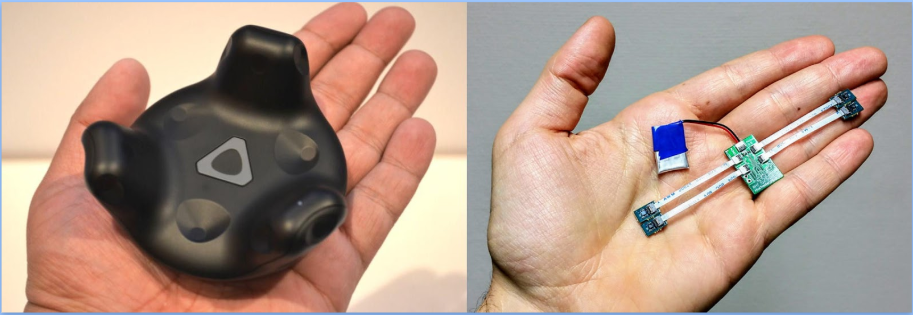
\includegraphics[scale=0.6]{Vivi_vs_HIVE.PNG}
	\caption{Vive Tracker et HIVE Tracker}
\end{figure}
	
Ce tracker est développé en collaboration dans 3 laboratoires : L'Universitat Politecnica de Valencia, le Kampff Lab à l'UCL et l'ISIR à la Sorbonne. Il a pour but de proposer un système de localisation 3D sous-millimétrique à prix bon marché.

\chapter{Simulation du système}

\section{Les lighthouses}

Les lighthouses sont vendues avec le matériel de réalité virtuel (VR) HTC Vive. Ce sont des petits systèmes fixes, qui permettent de repérer des accessoires de VR dans l'espace. Ils se positionnent en hauteur dans une pièces et doivent être visibles pour les manettes et le casque HTC Vive.\\

Le principe de fonctionnement des bases est le suivant : un broadcast (ou flash) puis un scann de l'espace.

\begin{figure}[h]
	\centering
	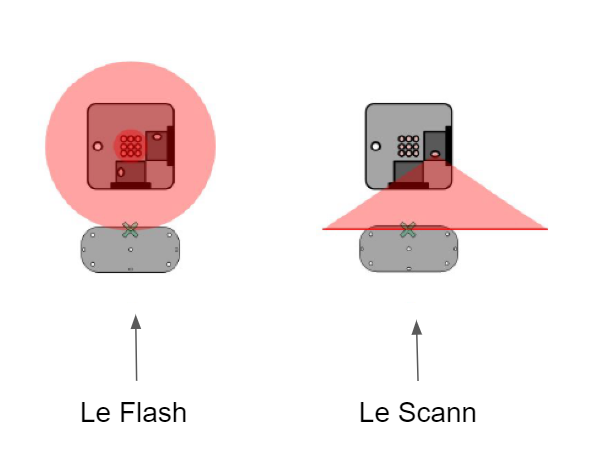
\includegraphics[scale=0.6]{Flash_scan.PNG}
	\caption{Le flash et le scann d'une lighthouse}
\end{figure}

Suivent un autre Flash puis un scann perpendiculaire au précédent. Ces étapes sont répétées ainsi de suite de manière très stable dans le temps.

\section{Le principe du positionnement}

\subsection{Le principe théorique}

Une photodiode, sensible à la lumière d'une lighthouse peut alors récupérer un timing de entre un broadcast et un scann. Deux timings, propositionnels aux angles de deux scann permettent d'obtenir un vecteur pointant la photodiode. Avec deux lighthouses, deux vecteurs sont obtenus. Connaissant la position et l'orientation des lighthouses, l'intersection de deux vecteurs est la position de notre photodiode

\subsubsection{L'intersection imparfaite}

Deux vecteurs non-colinéaires ne pouvant que très difficilement se croiser dans l'espace, il faut définir ce qu'est considéré comme leur intersection. Il s'agit alors du milieu du segment perpendiculaire au deux vecteurs.

\subsection{Autre principe}

Contrairement au principe énoncé précédemment, celui-ci se base sur l'hypothèse que les diodes sont sur un solide. De plus une seule lighthouse est nécessaire à ce positionnement.\\

Nous connaissons les distances séparant les photodiodes et un vecteur directeur au centre de chaque diode partant de la lighthouse. Par ailleurs nous cherchons les distance de chacune des photodiodes par rapport à la lighthouse. Pour le HIVE Tracker ayant 4 photodiodes, nous pouvons écrire 4 équations et avons 4 inconnues.\\

\begin{figure}[h]
	\centering
	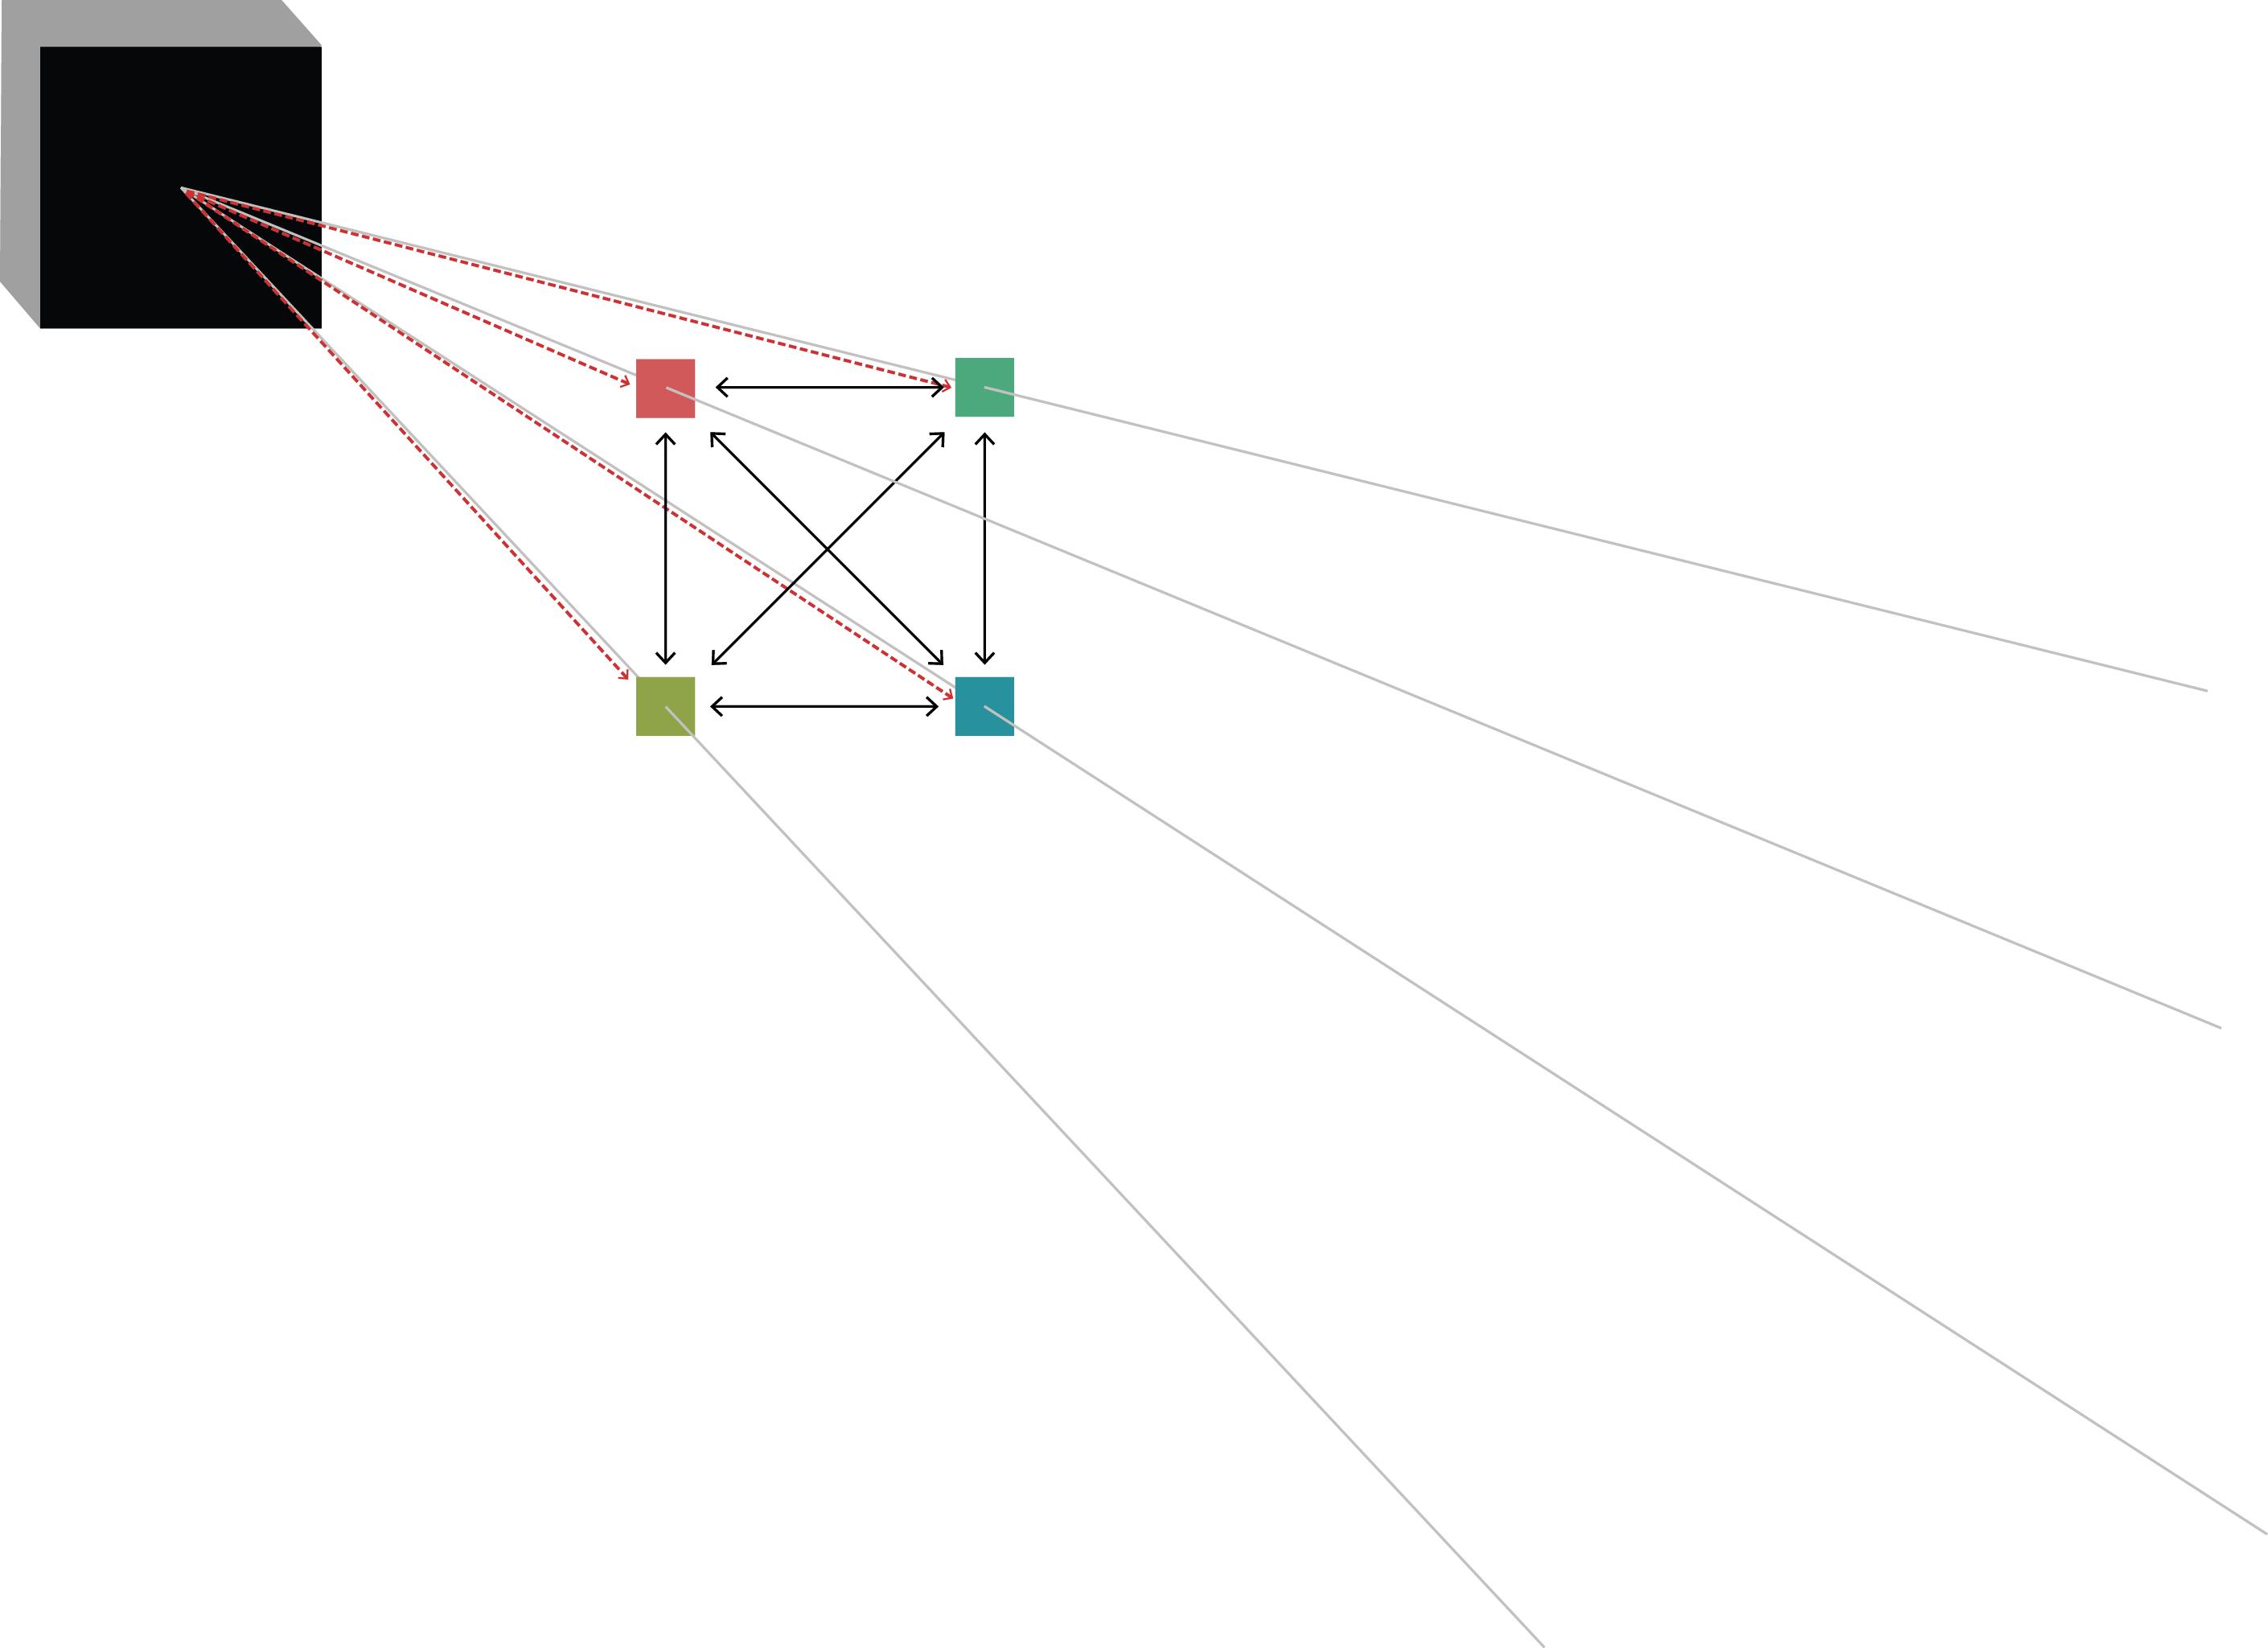
\includegraphics[scale=0.3]{one_LH.PNG}
	\caption{Positionnement à une seule lighthouse}
\end{figure}

\section{La simulation}

Blender étant un logiciel open source et multiplateforme nous avons fait le choix de l'utiliser pour réaliser une simulation reprenant les principes précédemment énoncés. Nous utiliserons sont moteur de jeu, le Blender Game Engine (BGE) qui est largement utilisé pour réaliser des simulations physiques ou faire des visualisations.\\

\subsubsection{Le scann dans la simulation}

Le scann des plan est réalisé en imposant un rotation à un plan. Lorsque la distance signée séparant le plan de l'objet courant change de signe, nous considéreront cet angle. Avec deux angles et deux lighthouses nous avons ainsi le principe de fonctionnement du système réel.

\subsubsection{Le principe de fonctionnement de la simulation}

La version finale de la simulation est faite comme un jeu vidéo. Un petit véhicule bleu peut être déplacé à l'aide du pavé numérique dans un salon. Sa position calculé est symbolisée par une sphère verte. Pour un soucis de compréhension du principe de fonctionnement du système HTC Vive, la vitesse de rotation qui réellement est de 120Hz, est ici ralentie. De plus les plans de scann sont colorés en rouge translucide.

\chapter{La fusion de capteurs}

\section{Les capteurs}

Les capteurs de mesure ayant tous des avantages et des inconvénient, le HIVE Tracker en embarque différents types. Nous essayerons plus tard de récupérer le meilleur de chacun.

\subsection{Les photodiodes}

La mesure réalisée par le photodiodes est très stable dans le temps, mais est aussi bruitée et a une plutôt faible fréquence de rafraichissement. De plus les photodiodes sont sensibles aux occlusions.\\

Le jitter observé impose un prétraitement des données mesurées. L'utilisation d'un simple filtre passe bas semble être un solution. Nous en étudierons deux types.

\subsection{La centrale inertielle}

Double intégration des accélérations mesurées par rapport au temps.

\section{Le filtre de Kalman}

\section{Le filtre de Madgwick}

Le filtre de Madgwick est principalement utilisé sur les données gyroscopique. Nous essayons ici de l'adapter pour l'utiliser sur le tracker. Il s'agit ici de réaliser une simple moyenne pondérée des donnée optiques et de celles de l'accéléromètre.

\chapter{L'implémentation}

\section{Le blocage de cardan}

\section{Conception d'une coque}

\subsection{Une coque de développement}

Il s'agit dans un premier temps de réaliser une structure modulable. Tout les composants du tracker doivent pouvoir être insérés et retirés facilement sans les endommager.

\subsection{Un coque optimisée}

Pour optimiser le positionnement des diodes dans l'espace, il faut que la coque les éloigne le plus possible les unes des autres. Cet arrangement est le tétraèdre. Une telle disposition nous assure même la visibilité d'au moins une diode, peu importe l'orientation de l'objet.



\chapter{Discussion}

\section{La caractérisation}




	
\chapter{Conclusion}

Ce stage fut ainsi une manière de découvrir le monde la recherche. Même si le problème sur lequel j'ai travaillé est théoriquement résolu, il est pratique difficile à mettre en œuvre et trouve de nombreuses imperfections. Même si certaines tâches se sont avérées plus courtes que prévues, l'ensemble du plan d'étude aura finalement été plus long à réaliser.\\









\end{document}